\chapter{Configuration}


\section{Runtime Configuration}\label{sec:runtime-config}

\subsection{SSL}

\subsubsection{Trusting Self-Signed Certificates}\label{sec:self-signed-certs}

While the \cxone system uses TLS certificates signed by a public CA, it is possible that
corporate proxies use certificates signed by a private CA. Private CA certificates must be imported
into the \cxoneflow container.

Each private CA certificate for import must meet the following criteria:

\begin{itemize}
    \item It must be in a file ending with the extension .crt.
    \item The contents of the file must be one certificate stored in the PEM format.
    \item All files containing private CA certificates must be mapped to the container path \texttt{/usr/local/share/ca-certificates}.
\end{itemize}


As an example, if using Docker, it is possible to map a single local file to a file in the container with this mapping 
option added to the container execution command line:

\begin{code}{Custom CA Mapping Option}{[Docker]}{}
-v $(pwd)/custom-ca.pem:/usr/local/share/ca-certificates/custom-ca.crt
\end{code}

\subsubsection{The \texttt{ssl-verify} Option}\label{sec:ssl-verify-general}

In the configuration YAML documentation, all of the \texttt{connection}
elements contain an optional \texttt{ssl-verify} setting.  This option
is generally useful to turn off SSL verification by setting it to \texttt{False}.
This can also be used to control which CA bundle is used for verification.

Omitting the \texttt{ssl-verify} setting should be sufficient for
most deployment cases.  If omitted, the container execution will use the default CA bundle
where any custom CAs are added as described in Section \ref{sec:self-signed-certs}.
The \texttt{ssl-verify} option can be set to an explicit path on the container
if there is a need to use a CA bundle other than the one provided by the OS.


\subsubsection{Configuring SSL for the \cxoneflowtext Endpoint}

Configuring the \cxoneflow endpoint for SSL communication requires an SSL certificate public/private key pair
and map the files to a location on the container.  The following environment variables must then be set in the
runtime environment:

\begin{table}[ht]
    \caption{SSL Environment Variables}
    \begin{tabularx}{\textwidth}{ll}
        \toprule
        \textbf{Variable} & \textbf{Description}\\
        \midrule
        \texttt{SSL\_CERT\_PATH} & \makecell[l]{The path to the server's SSL certificate in PEM format.}\\
        \midrule
        \texttt{SSL\_CERT\_KEY\_PATH} & \makecell[l]{The path to the certificate's unencrypted private key in PEM format.}\\
        \bottomrule
    \end{tabularx}
\end{table}

If your SSL certificate is self-signed, the certificate must also be imported as the CA as described
in Section \ref{sec:self-signed-certs}.  If the certificate is signed with a private CA, the private
CA must also be imported.  Failure to import a non-public signing CA for these types of certificates
will cause \cxoneflow startup failures.


\subsection{Runtime Control Environment Variables}

Environment variables can be set when the \cxoneflow container is executing to control some aspects of \cxoneflowns's operation.
Table \ref{tab:runtime-environment-vars} shows the operational environment variables and their meaning.

\begin{table}[ht]
    \caption{Runtime Control Environment Variables}\label{tab:runtime-environment-vars}
    \begin{tabularx}{\textwidth}{lccl}
        \toprule
        \textbf{Variable} & \textbf{Required} & \textbf{Default} & \textbf{Description}\\
        \midrule
        \texttt{CXONEFLOW\_WORKERS} & No & \texttt{max(\# of CPUs / 2, 1)} & \makecell[l]{The number of worker processes\\used for parallel execution. The\\maximum value will be\\set at \texttt{(\# of CPUs - 1)}}\\
        \midrule
        \texttt{LOG\_LEVEL} & No & \texttt{INFO} & \makecell[l]{The logging verbosity level.  Set to\\\texttt{DEBUG} for increased logging\\verbosity.}\\
        \midrule
        \texttt{CONFIG\_YAML\_PATH} & No & \texttt{/opt/cxone/config.yaml} & \makecell[l]{The path to the configuration\\YAML file.}\\
        \midrule
        \texttt{CXONEFLOW\_HOSTNAME} & No & \texttt{localhost} & \makecell[l]{The virtual hostname of the\\\cxoneflow endpoint.}\\
        \bottomrule
    \end{tabularx}
\end{table}


\newpage

\section{Operational Configuration}\label{sec:op-config}

The operational configuration uses a YAML file mapped at \texttt{/opt/cxone/config.yaml}
by default.  It is possible to map the \texttt{config.yaml} file to another location in the
container and adjust the path via the \texttt{CONFIG\_YAML\_PATH} environment variable.

\subsection{YAML Configuration Examples}

\subsubsection{Basic YAML Configurations}

The following example shows a minimal \cxoneflow configuration that defines the following:

\begin{enumerate}
    \item Files containing secrets are located at \texttt{/run/secrets}.
    \item One BitBucket Data Center SCM connection configuration to handle all webhook payloads
    POSTed to the \texttt{/bbdc} endpoint.
    \item One catch-all route for clone-urls using the regular expression \texttt{.*}
    \item The SCM's base URL located at \texttt{https://scm.corp.com}
    \item The shared secret used to validate webhook payloads located in the file \texttt{/run/secrets/scm-shared-secret}
    \item The API and clone authorization using a PAT in a file located at \texttt{/run/secrets/scm-token-secret}
    \item The CheckmarxOne tenant name of \texttt{mytenant}
    \item The CheckmarxOne API credentials using an \texttt{oauth} client with:
    \begin{enumerate}
        \item The client identifier located in the file \texttt{/run/secrets/my-oauth-id}
        \item The client secret located in the file \texttt{/run/secrets/my-oauth-secret}
    \end{enumerate}
    \item Using the CheckmarxOne multi-tenant US region IAM endpoint.
    \item Using the CheckmarxOne multi-tenant US region API endpoint.
\end{enumerate}

\begin{code}{Minimal YAML Configuration Example \#1}{[CxOne: oauth]}{[SCM: token auth]}
secret-root-path: /run/secrets

bbdc:
    - service-name: BitBucket DC
      repo-match: .*
      connection:
        base-url: https://scm.corp.com
        shared-secret: scm-shared-secret
        api-auth:
            token: scm-token-secret
      cxone:
        tenant: mytenant
        oauth:
            client-id: my-oauth-id
            client-secret: my-oauth-secret
        iam-endpoint: US
        api-endpoint: US
\end{code}

\pagebreak
\noindent\\An alternate minimal example using different authorization options:

\begin{code}{Minimal YAML Configuration Example \#2}{[CxOne: api-key]}{[SCM: basic/ssh auth]}
secret-root-path: /run/secrets

bbdc:
    - service-name: BitBucket DC
      repo-match: .*
      connection:
      base-url: https://scm.corp.com
      shared-secret: scm-shared-secret
      api-auth:
          username: scm-username-secret
          password: scm-password-secret
      clone-auth:
          ssh: scm-ssh-key-secret
      cxone:
        tenant: mytenant
        api-key: my-cxone-api-key
        iam-endpoint: US
        api-endpoint: US
\end{code}
    
\pagebreak
\noindent\\An alternate minimal example using for an Azure DevOps Enterprise
SCM:

\begin{code}{Minimal YAML Configuration Example \#2}{[CxOne: api-key]}{[SCM: basic/ssh auth]}
secret-root-path: /run/secrets

adoe:
    - service-name: MyADO
      repo-match: .*
      connection:
      base-url: https://scm.corp.com
      shared-secret: scm-shared-secret
      api-auth:
          username: scm-username-secret
          password: scm-password-secret
      clone-auth:
          ssh: scm-ssh-key-secret
      cxone:
        tenant: mytenant
        api-key: my-cxone-api-key
        iam-endpoint: US
        api-endpoint: US
\end{code}


\newpage
This example shows a \cxoneflow configuration explicitly setting default options in a service 
configuration for a single SCM.  The minimal examples leave several of these options as default.

The \texttt{scan-config} element has been added to this configuration to
demonstrate some of the controls that can be implemented over scan options.  In this
example, static Project and Scan tags are defined.  Also defined is the selection
of engines for the scan with some options defined as supported by the engine.
Documentation for the option keys can be found in the Checkmarx
\extlink{https://checkmarx.stoplight.io/docs/checkmarx-one-api-reference-guide/branches/main/f601dd9456e80-run-a-scan}{Scan REST API}
documentation and have the descriptions documented in the
\extlink{https://docs.checkmarx.com/en/34965-324311-settings-for-specific-scanners.html}{Scanners Settings}
documentation.

While there are options to apply scan configurations via \texttt{scan-config} elements, it is often the case that defining the scan configuration
in \cxoneflow will have undesirable results.  When defined in the \cxoneflow configuration, the configuration will explicitly override \cxone
tenant and project level default scan configurations.  Details about utilizing the \cxone configuration options for best results with \cxoneflow
can be found in Section \ref{sec:deployment-scan-defaults}.

\begin{code}{Full YAML Configuration Example}{[CxOne: oauth]}{[SCM: token auth]}
secret-root-path: /run/secrets
server-base-url: https://cxoneflow.mydomain.com:8443/

bbdc:
    - service-name: BitBucket DC
      repo-match: .*
      scan-config:
          default-scan-engines:
              sca:
                  exploitablePath: "True"
              sast:
                  presetName: ASA Premium
                  incremental: "False"
                  fastScanMode: "True"
                  filter: "!**/node_modules,!**/test*"
                  languageMode: multi
              kics:
              apisec:
          default-scan-tags:
              scan-service: BitBucket DC
          default-project-tags:
              onboarded-by: CxOneFlow
      connection:
          base-url: https://scm.corp.com
          shared-secret: scm-shared-secret
          timeout-seconds: 60
          retries: 3
          proxies:
            http: http://proxy.corp.com:8080
            https: http://proxy.corp.com:8080
          api-auth:
              token: scm-token-secret
      cxone:
          tenant: mytenant
          oauth:
              client-id: my-oauth-id
              client-secret: my-oauth-secret
          iam-endpoint: US
          api-endpoint: US
          timeout-seconds: 60
          retries: 3
          proxies:
            http: http://proxy.corp.com:8080
            https: http://proxy.corp.com:8080
\end{code}


\pagebreak
The next example shows a configuration where \cxoneflow has endpoint handlers for both
BitBucket Data Center and Azure DevOps Enterprise.  Each SCM is configured to handle multiple distinct
projects to demonstrate the use of multiple authentication methods.  All the SCM endpoints
orchestrate scans in a single \cxone tenant.

\begin{code}{Multi-SCM/Multi-Org YAML Configuration Example}{}{}
secret-root-path: /run/secrets
server-base-url: https://cxoneflow.mydomain.com:8443/
adoe-connection: &adoe-con
    base-url: http://adoe.scm.org/
    shared-secret: scm-shared-secret
bbdc-connection: &bbdc-con
    base-url: http://bbdc.scm.org
    shared-secret: scm-shared-secret
adoe:
    - service-name: ADO-EastCoast
        repo-match: .*East
        connection:
        <<: *adoe-con
        api-auth: 
            token: adoe-token-secret
        clone-auth: &clone-ssh
            ssh: ssh-priv-key
        cxone: &cxone
        tenant: my_tenant
        oauth:
            client-id: prod_client_id
            client-secret: prod_client_secret
        iam-endpoint: US
        api-endpoint: US
    - service-name: ADO-WestCoast
        repo-match: .*West
        connection:
        <<: *adoe-con
        api-auth:
            token: adoe-token-secret
        cxone: *cxone
bbdc:
    - service-name: BBDC-EastCoast
        repo-match: .*EAS
        connection:
        <<: *bbdc-con
        api-auth: 
            token: bbdc-token
        clone-auth: *clone-ssh
        cxone: *cxone
    - service-name: BBDC-WestCoast
        repo-match: .*WES
        connection:
        <<: *bbdc-con
        api-auth:
            token: bbdc-token
        cxone: *cxone
\end{code}



\subsubsection{Complex YAML Configurations using YAML Anchors}

For complex configurations, it is possible to use 
\extlink{https://docs.docker.com/compose/compose-file/10-fragments/}{YAML Anchors}
to avoid repeating some section definitions.  When using YAML anchors, it may be useful
to use a \extlink{https://onlineyamltools.com/convert-yaml-to-json}{YAML-to-JSON} conversion tool that shows the JSON generated from the YAML
definition

This example demonstrates defining common connection parameters that can be applied
to all connection definitions:


\begin{code}{Compacted Full YAML Configuration Example}{[CxOne: oauth]}{[SCM: token auth]}
secret-root-path: /run/secrets

my-connection-params: &common-connection-params
    timeout-seconds: 60
    retries: 3
    ssl-verify: True
    proxies:
    http: http://proxy.corp.com:8080
    https: http://proxy.corp.com:8080


bbdc:
    - service-name: BitBucket DC
      repo-match: .*
      scan-config:
          default-scan-engines:
              sca:
                  exploitablePath: "True"
              sast:
                  presetName: ASA Premium
                  incremental: "False"
                  fastScanMode: "True"
                  filter: "!**/node_modules,!**/test*"
                  languageMode: multi
              kics:
              apisec:
          default-scan-tags:
              scan-service: BitBucket DC
          default-project-tags:
              onboarded-by: CxOneFlow
      connection:
          base-url: https://scm.corp.com
          shared-secret: scm-shared-secret
          api-auth:
              token: scm-token-secret
          <<: *common-connection-params
      cxone:
          tenant: mytenant
          oauth:
              client-id: my-oauth-id
              client-secret: my-oauth-secret
          iam-endpoint: US
          api-endpoint: US
          <<: *common-connection-params
\end{code}


\noindent\\It is common to see a scenario where there are multiple organizations
using the same SCM instance.  A single \cxoneflow instance can be configured to accept
webhook events from all repos in each organization by using the \texttt{repo-match}
regular expression.  When a webhook payload is received, the \texttt{repo-match}
regular expression is applied to the clone URI until a match is found.

\noindent\\The example YAML below is used to demonstrate how \cxoneflow could be configured
for mulitple organizations in a single SCM. In the example, YAML anchors are utilized to 
re-use the common settings for each SCM organization.  Each organization, in this case, 
exists in the same SCM server and shares the same Checkmarx One instance.

\begin{code}{SCM Multi-Org YAML Configuration Example}{[CxOne: oauth]}{[SCM: token auth]}
secret-root-path: /run/secrets

my-connection-params: &common-connection-params
    timeout-seconds: 60
    retries: 3
    ssl-verify: True
    proxies:
    http: http://proxy.corp.com:8080
    https: http://proxy.corp.com:8080

bbdc:
    - service-name: BBDC-West
      repo-match: .*west
      scan-config: 
          default-scan-engines: &common-engine-config
              sca:
                  exploitablePath: "True"
              sast:
                  presetName: ASA Premium
                  incremental: "False"
                  fastScanMode: "True"
                  filter: "!**/node_modules,!**/test*"
                  languageMode: multi
              kics:
              apisec:
          default-scan-tags:
              scan-service: BBDC-West
          default-project-tags:
              onboarded-by: CxOneFlow
              region: West
      connection:
          base-url: https://scm.corp.com
          shared-secret: scm-west-org-shared-secret
          api-auth:
              token: scm-token-secret
          <<: *common-connection-params
      cxone: &cxone-config
          tenant: mytenant
          oauth:
              client-id: my-oauth-id
              client-secret: my-oauth-secret
          iam-endpoint: US
          api-endpoint: US
          <<: *common-connection-params
    - service-name: BBDC-East
      repo-match: .*east
      scan-config: 
          default-scan-engines: *common-engine-config
          default-scan-tags:
              scan-service: BBDC-East
          default-project-tags:
              onboarded-by: CxOneFlow
              region: East
      connection:
          base-url: https://scm.corp.com
          shared-secret: scm-east-org-shared-secret
          api-auth:
              token: scm-token-secret
          <<: *common-connection-params
      cxone: *cxone-config
\end{code}



\subsection{YAML Configuration Elements}\label{sec:yaml-config}

The organization of the YAML configuration is depicted in the tree below.  The description of each element
can be referenced by clicking the element.  Required elements are indicated in the tree; in general, if an
element that is not marked "required" is omitted, the feature that performs that operation is not invoked
for the configured service definition.

The \texttt{<root>} element indicates that elements directly under the root start at the farthest
left index of the line (this means a line position with an index of 0).  YAML elements that appear
under a parent element are intended to start at first tab stop past the parent element's tab stop.
Anchor elements may be defined at the root but must not clash with the names of any of the root elements.

Parts of the YAML tree have been split into individual trees to allow related elements to appear together.

\paragraph{YAML Root Elements}\label{sec:yaml-root}

\noindent\\

\dirtree{%
    .1 <root>.
    .2 \intlink{sec:yaml-secret-root-path}{secret-root-path} \DTcomment{[Required]}.
    .2 \intlink{sec:yaml-server-base-url}{server-base-url} \DTcomment{[Required]}.
    .2 \intlink{sec:yaml-scm-monikers}{<scm moniker>} \DTcomment{[At least 1 required: \textbf{bbdc}, \textbf{adoe}, \textbf{gh}, \textbf{gl}]}.
    .3 \intlink{sec:moniker-elements}{...see "YAML SCM Moniker Elements"}.
}

\pagebreak
\paragraph{YAML SCM Moniker Elements}\label{sec:moniker-elements}
\noindent\\The \texttt{<scm moniker>} element is a YAML list of dictionaries.  For a YAML list,
each entry is indented to the next tab after the parent and prefixed with a "\texttt{-}" (dash).
The elements in each list entry under \texttt{<scm moniker>} define key/value dictionary entries 
as the list entry.  Each list entry is referred to as a "service definition"
elsewhere in this document.\\\\

\dirtree{%
    .1 <root>.
    .2 \intlink{sec:yaml-scm-monikers}{<scm moniker>} \DTcomment{[Limited to: \textbf{bbdc}, \textbf{adoe}, \textbf{gh}, \textbf{gl}]}.
    .3 \intlink{sec:yaml-moniker-connection}{connection} \DTcomment{[Required]}.
    .4 \intlink{sec:connection-elements}{...see "YAML \texttt{connection} Elements"}.
    .3 \intlink{sec:yaml-moniker-cxone}{cxone} \DTcomment{[Required]}.
    .4 \intlink{sec:cxone-elements}{...see "YAML \texttt{cxone} Elements"}.
    .3 \intlink{sec:yaml-moniker-feedback}{feedback} \DTcomment{[Optional]}.
    .4 \intlink{sec:feedback-elements}{...see "YAML \texttt{feedback} Elements"}.
    .3 \intlink{sec:yaml-moniker-kickoff}{kickoff} \DTcomment{[Optional]}.
    .4 \intlink{sec:kickoff-elements}{...see "YAML \texttt{kickoff} Elements"}.
    .3 \intlink{sec:yaml-moniker-repo-match}{repo-match} \DTcomment{[Required]}.
    .3 \intlink{sec:yaml-moniker-resolver}{resolver} \DTcomment{[Optional]}.
    .4 \intlink{sec:resolver-elements}{...see "YAML \texttt{resolver} Elements"}.
    .3 \intlink{sec:yaml-moniker-scan-config}{scan-config} \DTcomment{[Optional]}.
    .4 \intlink{sec:scan-config-elements}{...see "YAML \texttt{scan-config} Elements"}.
    .3 \intlink{sec:yaml-moniker-service-name}{service-name} \DTcomment{[Required]}.
}

\pagebreak
\paragraph{YAML \texttt{connection} Elements}\label{sec:connection-elements}
\noindent\\

\dirtree{%
    .1 <root>.
    .2 \intlink{sec:yaml-scm-monikers}{<scm moniker>} \DTcomment{[Required: \textbf{bbdc}, \textbf{adoe}, \textbf{gh}, \textbf{gl}]}.
    .3 \intlink{sec:yaml-moniker-connection}{connection} \DTcomment{[Required]}.
    .4 \intlink{sec:yaml-connection-base-url}{base-url} \DTcomment{[Required]}.
    .4 \intlink{sec:yaml-connection-base-display-url}{base-display-url} \DTcomment{[Required for some SCMs]}.
    .4 \intlink{sec:yaml-connection-api-url-suffix}{api-url-suffix} \DTcomment{[Required for some SCMs]}.
    .4 \intlink{sec:yaml-connection-shared-secret}{shared-secret} \DTcomment{[Required]}.
    .4 \intlink{sec:yaml-generic-proxies}{proxies} \DTcomment{[Optional]}.
    .4 \intlink{sec:yaml-generic-retries}{retries} \DTcomment{[Optional] Default: 3}.
    .4 \intlink{sec:yaml-generic-ssl-verify}{ssl-verify} \DTcomment{[Optional] Default: True}.
    .4 \intlink{sec:yaml-generic-timeout-seconds}{timeout-seconds}\DTcomment{[Optional] Default: 60s}.
    .4 \intlink{sec:yaml-connection-api-auth}{api-auth} \DTcomment{[Required]}.
    .5 \intlink{sec:yaml-api-auth-app-private-key}{app-private-key} \DTcomment{[See element documentation]}.
    .5 \intlink{sec:yaml-api-auth-password}{password} \DTcomment{[See element documentation]}.
    .5 \intlink{sec:yaml-api-auth-token}{token} \DTcomment{[See element documentation]}.
    .5 \intlink{sec:yaml-api-auth-username}{username} \DTcomment{[See element documentation]}.
    .4 \intlink{sec:yaml-connection-clone-auth}{clone-auth} \DTcomment{[Optional] Default: \texttt{api-auth}}.
    .5 \intlink{sec:yaml-api-auth-password}{password} \DTcomment{[See element documentation]}.
    .5 \intlink{sec:yaml-clone-auth-ssh}{ssh} \DTcomment{[See element documentation]}.
    .5 \intlink{sec:yaml-clone-auth-ssh-port}{ssh-port} \DTcomment{[See element documentation]}.
    .5 \intlink{sec:yaml-api-auth-token}{token} \DTcomment{[See element documentation]}.
    .5 \intlink{sec:yaml-api-auth-username}{username} \DTcomment{[See element documentation]}.
}

\pagebreak
\paragraph{YAML \texttt{cxone} Elements}\label{sec:cxone-elements}
\noindent\\

\dirtree{%
    .1 <root>.
    .2 \intlink{sec:yaml-scm-monikers}{<scm moniker>} \DTcomment{[Required: \textbf{bbdc}, \textbf{adoe}, \textbf{gh}, \textbf{gl}]}.
    .3 \intlink{sec:yaml-moniker-cxone}{cxone} \DTcomment{[Required]}.
    .4 \intlink{sec:yaml-cxone-api-endpoint}{api-endpoint} \DTcomment{[Required]}.
    .4 \intlink{sec:yaml-cxone-api-key}{api-key} \DTcomment{[Required without oauth]}.
    .4 \intlink{sec:yaml-cxone-iam-endpoint}{iam-endpoint} \DTcomment{[Required]}.
    .4 \intlink{sec:yaml-cxone-oauth}{oauth} \DTcomment{[Required without api-key]}.
    .4 \intlink{sec:yaml-generic-proxies}{proxies} \DTcomment{[Optional]}.
    .4 \intlink{sec:yaml-generic-retries}{retries} \DTcomment{[Optional] Default: 3}.
    .4 \intlink{sec:yaml-generic-ssl-verify}{ssl-verify} \DTcomment{[Optional] Default: True}.
    .4 \intlink{sec:yaml-cxone-tenant}{tenant} \DTcomment{[Required]}.
    .4 \intlink{sec:yaml-generic-timeout-seconds}{timeout-seconds}\DTcomment{[Optional] Default: 60s}.
}


\pagebreak
\paragraph{YAML \texttt{feedback} Elements}\label{sec:feedback-elements}
\noindent\\


\dirtree{%
    .1 <root>.
    .2 \intlink{sec:yaml-scm-monikers}{<scm moniker>} \DTcomment{[Required: \textbf{bbdc}, \textbf{adoe}, \textbf{gh}, \textbf{gl}]}.
    .3 \intlink{sec:yaml-moniker-feedback}{feedback} \DTcomment{[Optional]}.
    .4 \intlink{sec:yaml-generic-amqp}{amqp} \DTcomment{[Optional] Default: container instance}.
    .5 \intlink{sec:yaml-generic-amqp-amqp-password}{amqp-password} \DTcomment{[Optional]}.
    .5 \intlink{sec:yaml-generic-amqp-amqp-url}{amqp-url} \DTcomment{[Required]}.
    .5 \intlink{sec:yaml-generic-amqp-amqp-user}{amqp-user} \DTcomment{[Optional]}.
    .5 \intlink{sec:yaml-generic-ssl-verify}{ssl-verify} \DTcomment{[Optional] Default: True}.
    .4 \intlink{sec:yaml-feedback-pull-request}{pull-request} \DTcomment{[Optional]}.
    .5 \intlink{sec:yaml-pull-request-enabled}{enabled} \DTcomment{[Optional] Default: False}.
    .4 \intlink{sec:yaml-feedback-scan-monitor}{scan-monitor} \DTcomment{[Optional]}.
    .5 \intlink{sec:yaml-scan-monitor-poll-backoff-multiplier}{poll-backoff-multiplier} \DTcomment{[Optional] Default: 2}.
    .5 \intlink{sec:yaml-scan-monitor-poll-interval-seconds}{poll-interval-seconds} \DTcomment{[Optional] Default: 90s}.
    .5 \intlink{sec:yaml-scan-monitor-poll-max-interval-seconds}{poll-max-interval-seconds} \DTcomment{[Optional] Default: 600s}.
    .5 \intlink{sec:yaml-scan-monitor-scan-timeout-hours}{scan-timeout-hours} \DTcomment{[Optional] Default: 48h}.
    .4 \intlink{sec:yaml-feedback-exclusions}{exclusions} \DTcomment{[Optional]}.
    .5 \intlink{sec:yaml-exclusions-severity}{severity} \DTcomment{[Optional]}.
    .5 \intlink{sec:yaml-exclusions-state}{state} \DTcomment{[Optional]}.
}

\pagebreak
\paragraph{YAML \texttt{kickoff} Elements}\label{sec:kickoff-elements}
\noindent\\

\dirtree{%
    .1 <root>.
    .2 \intlink{sec:yaml-scm-monikers}{<scm moniker>} \DTcomment{[Required: \textbf{bbdc}, \textbf{adoe}, \textbf{gh}, \textbf{gl}]}.
    .3 \intlink{sec:yaml-moniker-kickoff}{kickoff} \DTcomment{[Optional]}.
    .4 \intlink{sec:yaml-kickoff-max-concurrent-scans}{max-concurrent-scans} \DTcomment{[Optional]}.
    .4 \intlink{sec:yaml-kickoff-ssh-public-key}{ssh-public-key} \DTcomment{[Required]}.
}

\pagebreak
\paragraph{YAML \texttt{resolver} Elements}\label{sec:resolver-elements}
\noindent\\

\dirtree{%
    .1 <root>.
    .2 \intlink{sec:yaml-scm-monikers}{<scm moniker>} \DTcomment{[Required: \textbf{bbdc}, \textbf{adoe}, \textbf{gh}, \textbf{gl}]}.
    .3 \intlink{sec:yaml-moniker-resolver}{resolver} \DTcomment{[Optional]}.
    .4 \intlink{sec:yaml-generic-amqp}{amqp} \DTcomment{[Optional] Default: container instance}.
    .5 \intlink{sec:yaml-generic-amqp-amqp-password}{amqp-password} \DTcomment{[Optional]}.
    .5 \intlink{sec:yaml-generic-amqp-amqp-url}{amqp-url} \DTcomment{[Required]}.
    .5 \intlink{sec:yaml-generic-amqp-amqp-user}{amqp-user} \DTcomment{[Optional]}.
    .5 \intlink{sec:yaml-generic-ssl-verify}{ssl-verify} \DTcomment{[Optional] Default: True}.
    .3 \intlink{sec:yaml-resolver-allowed-agent-tags}{allowed-agent-tags} \DTcomment{[Required]}.
    .3 \intlink{sec:yaml-resolver-capture-resolver-logs}{capture-resolver-logs} \DTcomment{[Optional] Default: False}.
    .3 \intlink{sec:yaml-resolver-default-agent-tag}{default-agent-tag} \DTcomment{[Optional]}.
    .3 \intlink{sec:yaml-resolver-private-key}{private-key} \DTcomment{[Required]}.
    .3 \intlink{sec:yaml-resolver-resolver-tag-key}{resolver-tag-key} \DTcomment{[Optional] Default: resolver}.
    .3 \intlink{sec:resolver-scan-retries}{scan-retries}\DTcomment{[Optional] Default: 3}.
    .3 \intlink{sec:resolver-scan-timeout-seconds}]{scan-timeout-seconds}\DTcomment{[Optional] Default: 10800}.
}


\pagebreak
\paragraph{YAML \texttt{scan-config} Elements}\label{sec:scan-config-elements}
\noindent\\

\dirtree{%
    .1 <root>.
    .2 \intlink{sec:yaml-scm-monikers}{<scm moniker>} \DTcomment{[Required: \textbf{bbdc}, \textbf{adoe}, \textbf{gh}, \textbf{gl}]}.
    .3 \intlink{sec:yaml-moniker-scan-config}{scan-config} \DTcomment{[Optional]}.
    .4 \intlink{sec:yaml-scan-config-default-scan-engines}{default-scan-engines} \DTcomment{[Optional]}.
    .4 \intlink{sec:yaml-scan-config-default-project-tags}{default-project-tags} \DTcomment{[Optional]}.
    .4 \intlink{sec:yaml-scan-config-default-scan-tags}{default-scan-tags} \DTcomment{[Optional]}.
}


\subsubsection{YAML Element: Root}\label{sec:yaml-root}

The root elements of the YAML configuration are formatted to the left-most
position in the YAML file.  Anchor elements may be defined at the root but
must not clash with the names of any of the root elements.

\subsubsection{YAML Element: secret-root-path}\label{sec:yaml-secret-root-path}

A string that is the path to a directory that contains one or more files containing secret values.  The names to these files are 
referenced elsewhere in the YAML configuration file when used in a field that is a reference to a secret.

\subsubsection{YAML Element: server-base-url}\label{sec:yaml-server-base-url}
A string that is the base URL for the \cxoneflow endpoint.  This is used when creating feedback content that loads image elements.

\subsubsection{YAML Element: <scm moniker>}\label{sec:yaml-scm-monikers}

This is a moniker indicating the a list of service definitions for handling events from an SCM matching the name of the SCM
moniker.  Each service definition is a YAML dictionary of elements. The contents for each service definition dictionary 
have the same meaning unless otherwise specified.  At lease one SCM moniker with one configured service definition is required. 
The following SCM configuration monikers are currently supported:

\begin{itemize}
    \item \textbf{\texttt{bbdc}} for BitBucket Data Center webhook payloads targeting the \texttt{/bbdc}
    webhook payload receiver endpoint.
    \item \textbf{\texttt{adoe}} for Azure DevOps Enterprise or Cloud webhook payloads targeting the \texttt{/adoe}
    webhook payload receiver endpoint.
    \item \textbf{\texttt{gh}} for GitHub Enterprise or Cloud webhook payloads targeting the \texttt{/gh}
    webhook payload receiver endpoint.
\end{itemize}


\subsubsection{YAML Element: scan-config}\label{sec:yaml-moniker-scan-config}
A block element where the child elements define the default scan configuration for this service endpoint.

\subsubsection{YAML Element: service-name}\label{sec:yaml-moniker-service-name}
A moniker for the service definition. The moniker is used for logging and workflow purposes.

\subsubsection{YAML Element: repo-match}\label{sec:yaml-moniker-repo-match}
A regex applied to the source repository.  If the webhook payload has
a clone URL that matches the regex, this service definition is used to orchestrate the scanning.

\subsubsection{YAML Element: connection}\label{sec:yaml-moniker-connection}
A block element where the child elements define the SCM connection parameters for this service definition.

\subsubsection{YAML Element: cxone}\label{sec:yaml-moniker-cxone}
A block element where the child elements define the connection configuration for the \cxone API. 

\subsubsection{YAML Element: feedback}\label{sec:yaml-moniker-feedback}
A block element where the child elements define the configuration for feedback workflows. 

\subsubsection{YAML Element: resolver}\label{sec:yaml-moniker-resolver}
A block element where the child elements define the configuration for support of resolver agents. 


\subsubsection{YAML Element: default-scan-engines}\label{sec:yaml-scan-config-default-scan-engines}

A dictionary YAML element that follows the format \texttt{<engine-name>:<engine config option dictionary>}
corresponding to the configuration element of the
\href{https://checkmarx.stoplight.io/docs/checkmarx-one-api-reference-guide/branches/main/f601dd9456e80-run-a-scan}{\cxonetext scan API}.
Any static engine configuration supported by an engine can be defined here.  If a configuration is defined that is not supported
by the engine, scans may fail to start.

\subsubsection{YAML Element: default-scan-tags}\label{sec:yaml-scan-config-default-scan-tags}
A dictionary YAML element containing static key:value pairs that are assigned to each scan.

\subsubsection{YAML Element: default-project-tags}\label{sec:yaml-scan-config-default-project-tags}
A dictionary YAML element containing static key:value pairs that are assigned\\to each project upon project creation.


\subsubsection{YAML Element: <scm moniker>.cxone.api-endpoint}\label{sec:yaml-cxone-api-endpoint}
This can be a fully qualified domain name of a server or a multi-tenant API endpoint moniker as described in Appendix \ref{sec:endpoint-monikers}.

\subsubsection{YAML Element: <scm moniker>.cxone.api-key}\label{sec:yaml-cxone-api-key}
If not defined, the \texttt{oauth} element must be defined. The value specifies a file name found under the path defined by \texttt{secret-root-path}.

\subsubsection{YAML Element: <scm moniker>.cxone.iam-endpoint}\label{sec:yaml-cxone-iam-endpoint}
This can be a fully qualified domain name of a server or a multi-tenant IAM endpoint moniker as described in Appendix \ref{sec:endpoint-monikers}.

\subsubsection{YAML Element: <scm moniker>.cxone.oauth}\label{sec:yaml-cxone-oauth}
If not defined, the \texttt{api-key} element must be defined. This contains two required elements
\texttt{client-id} and \texttt{client-secret} where each value corresponds to a file name found under the path defined by \texttt{secret-root-path}. 

\subsubsection{YAML Element: <scm moniker>.cxone.tenant}\label{sec:yaml-cxone-tenant}
The name of the \cxone tenant.


\chapter{Workflows}\label{sec:workflows}


\section{Overview}

When webhook events are received by \cxoneflow, the content of the event
payload is evaluated to determine if a scan should be started.  If a scan
is started, a background workflow executes that monitors the scan progress.
When the scan is completed and produces results, the end of the workflow
will transform the results for the purpose of presenting them to the user
for evaluation.

This section describes the workflows as implemented by \cxoneflow.  Integration
with the workflows to perform parallel or replacement activities is possible
by utilizing the internal workflow messaging. It is possible, via configuration,
to turn off the feedback output and the messaging workflows still execute; this
allows integration scenarios that replace default feedback output.  If the
feedback output remains enabled via configuration, this allows integration
scenarios for customized workflows to execute in parallel with feedback
output implemented in \cxoneflow. Please see Appendix 
\ref{sec:amqp-workflow-orch} for details related to workflow integration.

The messaging mechanism is used to ensure workflows execute to the end
and can recover in the event of an error or abnormal program end.  Figure
\ref{fig:recovery-flowchart} shows the algorithm that is used
in all workflows handle error recovery.  A system restart when \cxoneflow
is not deployed in a high-availability configuration will cause running workflows
to be ended without the ability to recover.  To deploy \cxoneflow so that
a workflows can recover after a system restart, please see
Appendix \ref{sec:high-availability} for details about deploying \cxoneflow
in a high-availability configuration.


\begin{figure}[ht]
    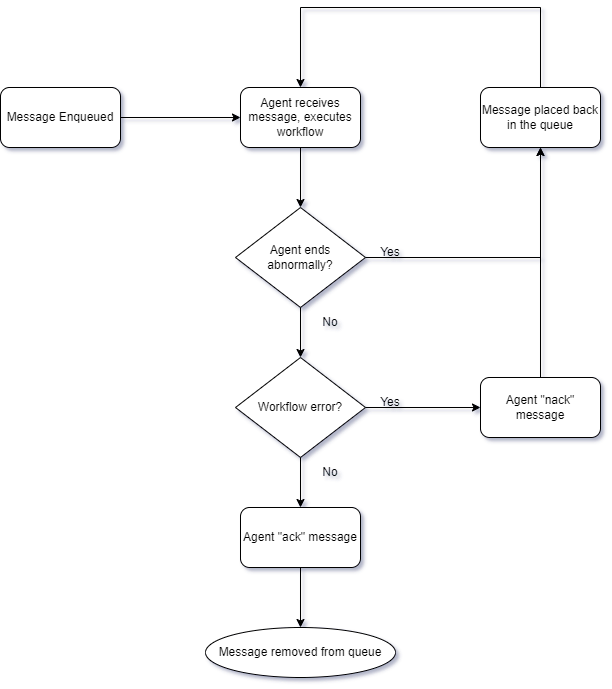
\includegraphics[width=\textwidth]{graphics/cxoneflow-diagrams-Recovery Algorithm.png}
    \caption{Workflow Recovery Algorithm}
    \label{fig:recovery-flowchart}
\end{figure}



\section{Scan Monitoring}

A scan in CheckmarxOne can be performed using one or more different scan engines.
A scan that has been completed will generally decide the next step in the workflow.
Keep in mind that a "completed" scan may mean the scan ended with any of the
following outcomes:

\begin{itemize}
    \item Scans for all requested engines completed successfully, each having zero
    or more results.
    \item The scan may have failed with no engines ever having started a scan.
    \item The scan may have partially failed where one or more engines successfully
    completed a scan and one or more engines had a scan failure.
    \item The scan may have been cancelled before any engine produced results.
    \item The scan may have been cancelled after one or more engines produced
    results but before all the engines were able to produce results.
\end{itemize}

When the scan is completed (which doesn't imply that it was successful), a message
is enqueued that starts the next step in the workflow.  
Figure \ref{fig:polling-flowchart} shows the scan polling algorithm that is followed
to determine when to enqueue a message that starts the next step in the workflow.

\begin{figure}[ht]
    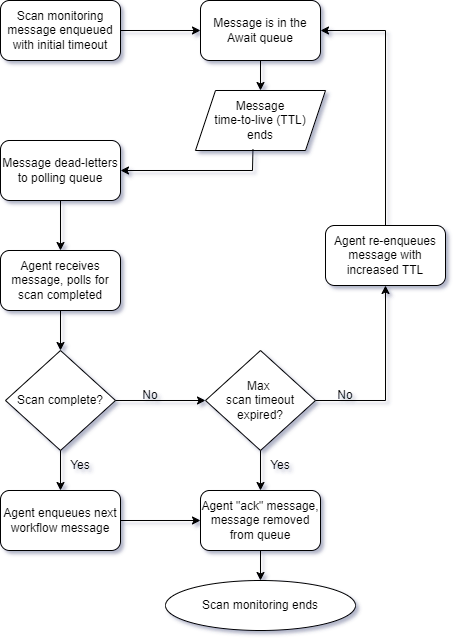
\includegraphics[width=\textwidth, scale=.75]{graphics/cxoneflow-diagrams-Polling Algorithm.png}
    \caption{Scan Polling Algorithm}
    \label{fig:polling-flowchart}
\end{figure}

\section{Annotation Workflow}\label{sec:annotation-workflow}

The annotation workflow is intended to perform any type of operations that
would inform a user of the following scan dispositions:

\begin{itemize}
    \item Started
    \item Cancelled
    \item Failed
\end{itemize}

\noindent\\The messaging workflow is currently very simple and follows the algorithm
shown in Figure \ref{fig:recovery-flowchart}.

\section{Pull Request Feedback Workflow}\label{sec:pull-request-workflow}

The pull request feedback workflow is invoked when a scan completes with the
following conditions:

\begin{itemize}
    \item A scan is fully completed on all requested scan engines.
    \item A scan is in the \texttt{Partial} result state with no
    engines currently running a scan.
\end{itemize}

The feedback workflow messaging follows the algorithm shown in
Figure \ref{fig:recovery-flowchart}.  The feedback that is emitted
for pull-request feedback is a summary of components found in the
\href{https://docs.checkmarx.com/en/34965-182434-checkmarx-one-reporting.html}{Improved Scan Report}
as generated by the
\href{https://checkmarx.stoplight.io/docs/checkmarx-one-api-reference-guide/branches/main/7bf86350cfe72-create-a-report}{"create a report"}
CheckmarxOne API.  Some results can be excluded via configuration,
as described in Section \ref{sec:exclusions-element}.  If the results of a particular
engine are not included in the Improved Scan Report, they are not available for
publication in the feedback comment.

\subsection{Pull Request Comment Contents}

Each source control system will impose a maximum size for content written in
a pull request comment.  Since scans can produce an unpredictable number of
results for each engine scanned, it is possible that a full itemized
summary of results in a pull request comment will exceed the maximum comment
size.  \cxoneflow will write the full itemized summary of results if the
content size is less than the maximum comment content size.  In the event that
the maximum comment content size would be exceeded, a simple count of
vulnerabilities by severity and engine is written as the comment content.


\subsubsection{Header}

An example header of the pull-request comment is shown in Figure
\ref{fig:pr-header-section}.  It contains a link to the scan
and an indicator of the scan status of the selected engines.  An indicator
of a red "X" next to an engine indicates the scan status of anything other
than successful completion of the scan running on that engine.

\begin{figure}[ht]
    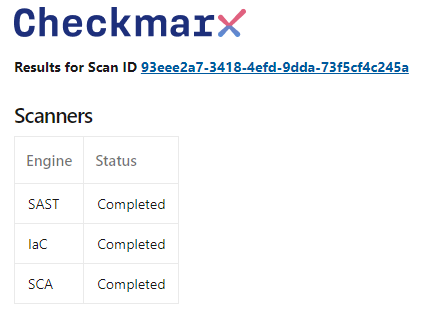
\includegraphics[width=\textwidth]{graphics/pr-header.png}
    \caption{Pull-Request Comment Header}
    \label{fig:pr-header-section}
\end{figure}

\subsubsection{Summary of Vulnerabilities}

An example summary of vulnerability counts by severity and engine 
is shown in Figure \ref{fig:pr-summary}.  The calculated counts will not
include vulnerabilities marked as "Not Exploitable".  Severities that
are configured for exclusions, as documented in Section
\ref{sec:exclusions-element}, are not included in the table.  When no 
vulnerabilities of a given severity with a status other than 
"Not Exploitable" are found, the count is indicated by "N/R" (none reported).


The counts for SCA scans only reflect the reported vulnerabilities in the
Risks tab of the SCA results viewer.  The count will differ from the summary
of SCA results shown when selecting a scan in Scan History; the scan
history view shows a combined count of all categories of SCA results.

\begin{figure}[ht]
    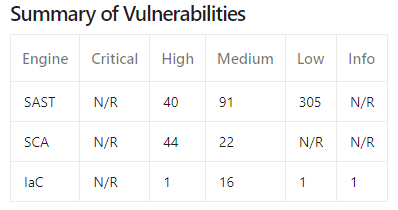
\includegraphics[width=\textwidth]{graphics/pr-summary.png}
    \caption{Pull-Request Summary Count by Severity and Engine}
    \label{fig:pr-summary}
\end{figure}


\subsubsection{SAST Results}

An example of the SAST result summary written to the pull-request comment
is shown in Figure
\ref{fig:pr-sast-section}.  The name of the issue is a link to a detailed
explanation of the vulnerability that includes remediation advice.  A
link to the line of the source code leads to the source file located in the
repository.  The Checkmarx Insight link opens the triage view for the vulnerable
data flow.

\begin{figure}[ht]
    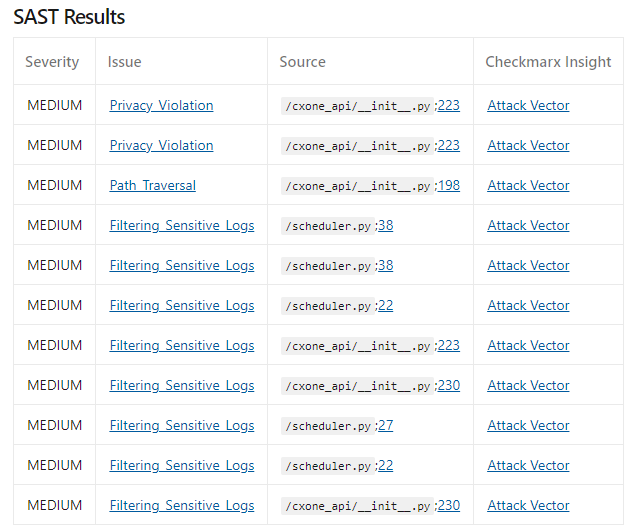
\includegraphics[width=\textwidth]{graphics/pr-sast.png}
    \caption{Pull-Request Comment SAST Results}
    \label{fig:pr-sast-section}
\end{figure}

\subsubsection{SCA Results}

An example of the SCA result summary written to the pull-request comment
is shown in Figure
\ref{fig:pr-sca-section}.  The Checkmarx Insight link opens the triage view 
for the vulnerable package. 

\begin{figure}[ht]
    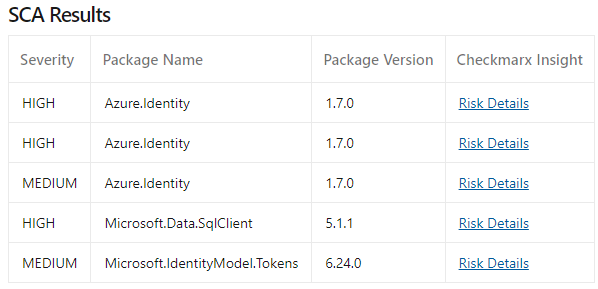
\includegraphics[width=\textwidth]{graphics/pr-sca.png}
    \caption{Pull-Request Comment SCA Results}
    \label{fig:pr-sca-section}
\end{figure}

\subsubsection{IAC Results}

An example of the IAC result summary written to the pull-request comment
is shown in Figure
\ref{fig:pr-iac-section}. A
link to the line of the source code leads to the source file located in the
repository.  The Checkmarx Insight link opens the triage view for the vulnerable
configuration.

\begin{figure}[ht]
    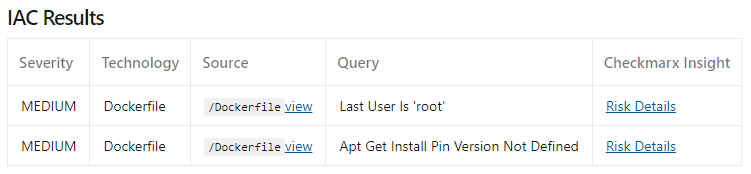
\includegraphics[width=\textwidth]{graphics/pr-iac.png}
    \caption{Pull-Request Comment IaC Results}
    \label{fig:pr-iac-section}
\end{figure}

\subsubsection{Resolved Issues}

An example of the Resolved Issues summary written to the pull-request comment
is shown in Figure
\ref{fig:pr-resolved-section}. This section appears only if a scan results in
some of the issues are found to have been resolved by a new scan.
The Checkmarx Insight link opens the triage view for the vulnerable
data flow.

\begin{figure}[ht]
    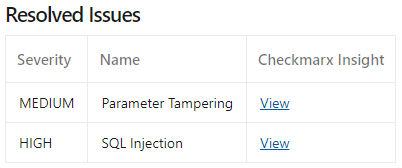
\includegraphics[width=\textwidth]{graphics/pr-resolved.png}
    \caption{Pull-Request Comment Resolved Section}
    \label{fig:pr-resolved-section}
\end{figure}


\subsubsection{YAML Element: max-concurrent-scans}\label{sec:yaml-kickoff-max-concurrent-scans}
The number of concurrent kickoff scans that the kickoff workflow will allow for the service definition.
The maximum does not include running scans that were initiated using other methods. If the
maximum concurrent kickoff scans is running, the server will indicate to the client that it needs
try submitting a scan later.

The default value is 3 if the element is not configured.  Values less than 1 will be
set to 1; values more than 10 will force the maximum number of concurrent kickoff scans
to 10.  


\subsubsection{YAML Element: ssh-public-key}\label{sec:yaml-kickoff-ssh-public-key}
The value specifies a file name found under the path defined by \texttt{secret-root-path}
containing an SSH public key as generated by \texttt{ssh-keygen}.  The associated private key will be
held securely by clients of the Kickoff API.


\subsubsection{YAML Element: enabled}\label{sec:yaml-pull-request-enabled}
Defaults to \texttt{False}.  If set to \texttt{True}, the feedback workflow for Pull Requests is executed upon completion of a scan generated by
a Pull Request. See Section \ref{sec:pull-request-workflow} for details about the Pull Request feedback workflow.




\subsubsection{YAML Element: poll-interval-seconds}\label{sec:yaml-scan-monitor-poll-interval-seconds}
The number of seconds to use in calculating scan status polling time intervals.


\subsubsection{YAML Element: poll-max-interval-seconds}\label{sec:yaml-scan-monitor-poll-max-interval-seconds}
The maximum polling interval seconds.


\subsubsection{YAML Element: poll-backoff-multiplier}\label{sec:yaml-scan-monitor-poll-backoff-multiplier}
A scalar used to increase the scan polling interval after each poll execution.

\subsubsection{YAML Element: scan-timeout-hours}\label{sec:yaml-scan-monitor-scan-timeout-hours}
The number of hours before a feedback workflow aborts waiting for a scan to finish executing.  Set to 0 to wait forever.

\subsubsection{YAML Element: state }\label{sec:yaml-exclusions-state}
A YAML list element that supports the following values:

\begin{itemize}
  \item Not Exploitable
  \item To Verify
  \item Proposed Not Exploitable
  \item Confirmed
  \item Urgent
\end{itemize}



\subsubsection{YAML Element: severity}\label{sec:yaml-exclusions-severity}
A YAML list element that supports the following values:

\begin{itemize}
  \item Critical
  \item High
  \item Medium
  \item Low
  \item Info
\end{itemize}



\subsubsection{YAML Element: base-url}\label{sec:yaml-connection-base-url}
The base url of the SCM server's API endpoint. This should be the root URL for the API that can be used when composing all
API calls related to the source of the received webhook event.

\subsubsection{YAML Element: base-display-url}\label{sec:yaml-connection-base-display-url}
An optional URL for use when composing links as part of an information display such as pull-request
feedback. Most SCMs will not require this setting.

\subsubsection{YAML Element: api-url-suffix}\label{sec:yaml-connection-api-url-suffix}
An optional API URL suffix used when composing API request URLs. Most SCMs will not require this setting.

\subsubsection{YAML Element: shared-secret}\label{sec:yaml-connection-shared-secret}
The shared secret configured in the SCM used to sign webhook payloads. The shared secret must meet the
following minimum criteria: 

\begin{itemize}
  \item 20 characters long
  \item contains at least 3 numbers
  \item contains at least 3 upper-case letters
  \item contains at least 2 special characters
\end{itemize}

\subsubsection{YAML Element: api-auth}\label{sec:yaml-connection-api-auth}
A YAML dictionary of SCM authorization options for using the API.

The authorization methods for \texttt{api-auth} 
are used to communicate with the SCM's API and can often be used for cloning repositories.  The
main difference between \texttt{api-auth} and \texttt{clone-auth} is that API access generally
does not support SSH authorization. If there is a need to clone using SSH, configure the SSH
authorization under the \texttt{clone-auth} element.  

The elements of \texttt{api-auth} are required depending on the type of authorization that
needs to be performed.

\subsubsection{YAML Element: clone-auth}\label{sec:yaml-connection-clone-auth}
Defines authorization options for performing clones when it differs from authorization for API requests.

The \texttt{clone-auth} element is optional;  if not provided, the connection information defined
in \texttt{api-auth} will be used.
\subsubsection{YAML Element: token}\label{sec:yaml-api-auth-token}
The value specifies a file name found under the path defined by \texttt{secret-root-path} 
containing a Personal Access Token (PAT).  This is required for token authorization.  This can
be combined with the \texttt{username} element.


\subsubsection{YAML Element: username}\label{sec:yaml-api-auth-username}

\textbf{For Token Authorization}
The value specifies a file name found under the path defined by \texttt{secret-root-path} containing a username associated with the PAT.
This is optional and only used during cloning; if not supplied, the default username of \texttt{git} is used. Can be combined with 
the \texttt{token} element.


\textbf{For Basic Authorization}\footnote{Many SCMs no longer support basic authorization.}
The value specifies a file name found under the path defined by \texttt{secret-root-path} containing the username associated with the account used
for authorization.  This element can be supplied with the \texttt{password} element.

\subsubsection{YAML Element: password}\label{sec:yaml-api-auth-password}
The value specifies a file name found under the path defined by \texttt{secret-root-path} 
containing a password associated with the username found in the \texttt{username} element.  
This is required for basic authorization if basic authorization is supported by the SCM instance.
This can be combined with the \texttt{username} element.


\subsubsection{YAML Element: app-private-key}\label{sec:yaml-api-auth-app-private-key}
The value specifies a file name found under the path defined by \texttt{secret-root-path} containing a private key used
when obtaining application authorization. 

Application Authorization is available for use with select SCM types. Refer to Part \ref{part:scms} for details about SCMs
that support this type of authorization. When using Application Authorization, there is typically not a need to provide a separate 
method of authorization for cloning defined in the \texttt{clone-auth} element. 

\subsubsection{YAML Element: ssh}\label{sec:yaml-clone-auth-ssh}
The value specifies a file name found under the path defined by \texttt{secret-root-path} containing an unencrypted private SSH key.

\subsubsection{YAML Element: ssh-port}\label{sec:yaml-clone-auth-ssh-port}
This optional value specifies the port used for SSH cloning if the SCM is not using port 22
and does not automatically include it in the clone URL.


\chapter{Resolver Workflows}\label{sec:resolver-workflows}

\section{Overview}
For any scan invoked by \cxoneflow\space when \hyperref[sec:resolver-elements]{configured to use resolver}, 
a "deferred" scan is enqueued with the message queue to run a resolver scan.  The deferred scan is handed over
to a distributed resolver agent that clones the code and executes \scaresolver.  The \scaresolver results are
then sent back to the \cxoneflow endpoint server to submit for scan along with the code.  This section details
exchange, queue, and workflow logic of this process.


\section{Deferred Scan Workflow}

The \cxoneflow endpoint logs will indicate scans are deferred when the algorithm for event handling
determines a resolver scan is needed.  Figure \ref{fig:deferred-scan-flowchart} shows the deferred-scan
workflow algorithm that is followed to determine when to request a deferred scan.  

\begin{figure}[ht]
  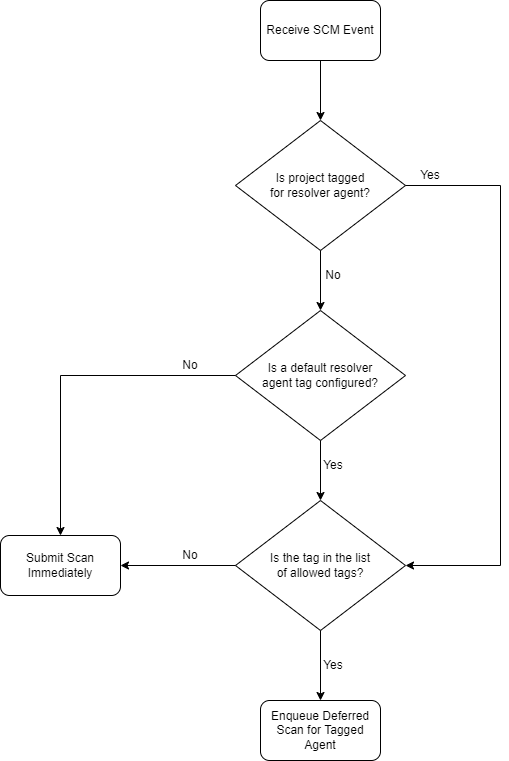
\includegraphics[width=\textwidth]{graphics/cxoneflow-diagrams-Deferred Scan Algorithm.png}
  \caption{Deferred Scan Algorithm}
  \label{fig:deferred-scan-flowchart}
\end{figure}


\section{Post Deferred Scan Workflow}

When the \scaresolver scan is complete, the distributed resolver agent will send the results
to the \cxoneflow endpoint for submission in the \cxone scan.  Scans with \scaresolver can
complete successfully or end with failure.

If the \scaresolver scan is successful, the results of the 
\href{https://docs.checkmarx.com/en/34965-19199-running-scans-using-checkmarx-sca-resolver.html#UUID-af718204-6dfc-2b27-439e-419b9157d364_id_RunningScansUsingCheckmarxSCAResolver-CheckmarxSCAResolverModes}{offline}
scan are submitted as part of the \cxone scan.  If the \scaresolver scan fails (for any reason), the \cxone scan is submitted for server-side dependency resolution.
Figure \ref{fig:post-deferred-scan-flowchart} shows the post-deferred-scan workflow algorithm.

\begin{figure}[ht]
  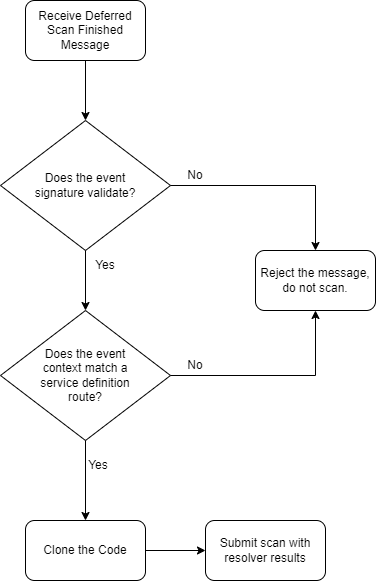
\includegraphics[width=\textwidth]{graphics/cxoneflow-diagrams-Post Deferred Scan Algorithm.png}
  \caption{Post Deferred Scan Algorithm}
  \label{fig:post-deferred-scan-flowchart}
\end{figure}




\subsubsection{YAML Element: amqp}\label{sec:yaml-generic-amqp}
The connection parameters for an AMQP endpoint used for workflow orchestration and resolver agent coordination. 
If not set, the internal RabbitMQ instance in the \cxoneflow container is used by default.

\subsubsection{YAML Element: amqp-url}\label{sec:yaml-generic-amqp-amqp-url}
This can be one of the following values:

\begin{itemize}
  \item The AMQP/AMQPS URL for the AMQP endpoint.
  \item The name of a file container a secret located at the path defined by \texttt{secret-root-path}.
\end{itemize}


\subsubsection{YAML Element: amqp-user}\label{sec:yaml-generic-amqp-amqp-user}
If the user name is not included in the AMQP URL, the provided value corresponds to a file name found under
the path defined by \texttt{secret-root-path}.

\subsubsection{YAML Element: amqp-password}\label{sec:yaml-generic-amqp-amqp-password}
If the password is not included in the AMQP URL, the provided value corresponds to a file name found
under the path defined by \texttt{secret-root-path}.


\subsubsection{YAML Element: ssl-verify}\label{sec:yaml-generic-ssl-verify}
See discussion in Section \ref{sec:ssl-verify-general}.  Defaults to True using the OS trusted CA certificates.

\subsubsection{YAML Element: timeout-seconds}\label{sec:yaml-generic-timeout-seconds}
The number of seconds before a request for API results times out.

\subsubsection{YAML Element: retries}\label{sec:yaml-generic-retries}
The number of retries when the request fails.


\subsubsection{YAML Element: proxies}\label{sec:yaml-generic-proxies}
A YAML dictionary of \texttt{<scheme>:<url>} pairs to use a proxy server for requests. 
For a format of key/value pairs, see: \extlink{https://requests.readthedocs.io/en/latest/user/advanced/\#proxies}{Python "requests" proxies}.










